\documentclass[border=4pt]{standalone}

\usepackage{amsmath}
\usepackage{tikz}
\usepackage{mathdots}
\usepackage{yhmath}
\usepackage{cancel}
\usepackage{color}
\usepackage{siunitx}
\usepackage{array}
\usepackage{multirow}
\usepackage{amssymb}
\usepackage{gensymb}
\usepackage{tabularx}
\usepackage{booktabs}
\usetikzlibrary{fadings}
\usetikzlibrary{patterns}


\begin{document}
 



\tikzset{every picture/.style={line width=0.75pt}} %set default line width to 0.75pt        

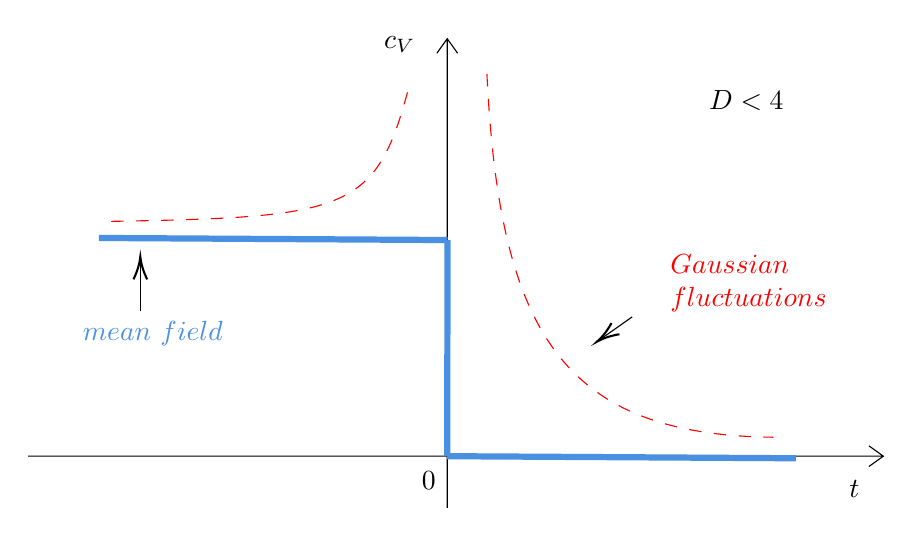
\begin{tikzpicture}[x=0.75pt,y=0.75pt,yscale=-1,xscale=1]
%uncomment if require: \path (0,300); %set diagram left start at 0, and has height of 300

%Shape: Axis 2D [id:dp501093661208917] 
\draw  (98,243.14) -- (510,243.14)(299.88,42) -- (299.88,268) (503,238.14) -- (510,243.14) -- (503,248.14) (294.88,49) -- (299.88,42) -- (304.88,49)  ;
%Straight Lines [id:da13881414446900964] 
\draw [color={rgb, 255:red, 74; green, 144; blue, 226 }  ,draw opacity=1 ][line width=2.25]    (132,138) -- (300,139) ;


%Straight Lines [id:da09025717984492121] 
\draw [color={rgb, 255:red, 74; green, 144; blue, 226 }  ,draw opacity=1 ][line width=2.25]    (299.88,243.14) -- (467.88,244.14) ;


%Straight Lines [id:da4929192701914391] 
\draw [color={rgb, 255:red, 74; green, 144; blue, 226 }  ,draw opacity=1 ][line width=2.25]    (300,139) -- (299.88,243.14) ;


%Curve Lines [id:da7736843369468178] 
\draw [color={rgb, 255:red, 255; green, 0; blue, 0 }  ,draw opacity=1 ] [dash pattern={on 4.5pt off 4.5pt}]  (138,130) .. controls (254,128) and (266,125) .. (282,63) ;


%Curve Lines [id:da4281079652632538] 
\draw [color={rgb, 255:red, 255; green, 0; blue, 0 }  ,draw opacity=1 ] [dash pattern={on 4.5pt off 4.5pt}]  (319,59) .. controls (325,183) and (355,233) .. (457,234) ;


%Straight Lines [id:da6218571705711013] 
\draw    (152,173) -- (152,149) ;
\draw [shift={(152,147)}, rotate = 450] [color={rgb, 255:red, 0; green, 0; blue, 0 }  ][line width=0.75]    (10.93,-3.29) .. controls (6.95,-1.4) and (3.31,-0.3) .. (0,0) .. controls (3.31,0.3) and (6.95,1.4) .. (10.93,3.29)   ;

%Straight Lines [id:da19245040250997714] 
\draw    (389,176) -- (373.63,186.85) ;
\draw [shift={(372,188)}, rotate = 324.78] [color={rgb, 255:red, 0; green, 0; blue, 0 }  ][line width=0.75]    (10.93,-3.29) .. controls (6.95,-1.4) and (3.31,-0.3) .. (0,0) .. controls (3.31,0.3) and (6.95,1.4) .. (10.93,3.29)   ;


% Text Node
\draw (291,255) node    {$0$};
% Text Node
\draw (496,259) node    {$t$};
% Text Node
\draw (277,45) node    {$c_{V}$};
% Text Node
\draw (158,184) node  [color={rgb, 255:red, 74; green, 144; blue, 226 }  ,opacity=1 ]  {$mean\ field$};
% Text Node
\draw (445,160) node  [color={rgb, 255:red, 255; green, 0; blue, 0 }  ,opacity=1 ]  {$ \begin{array}{l}
Gaussian\\
fluctuations
\end{array}$};
% Text Node
\draw (444,72) node    {$D< 4$};


\end{tikzpicture}

\end{document}
